
	\documentclass{article}
	\usepackage{amsmath,amssymb}
	\usepackage[inline]{enumitem}
	\usepackage{blindtext}
	\usepackage{booktabs}
	\usepackage{graphicx}
	\usepackage{xcolor}
	\usepackage[vmargin = 1.5in, top = 1in, bottom = 1.2in, letterpaper]{geometry}
	\usepackage{listings}
	\usepackage{courier}
	\usepackage{bm}
	\lstset{
	basicstyle = \small\tt,
	keywordstyle = \tt\color{blue},
	commentstyle = \it\color[cmyk]{1,0,1,0},
	stringstyle = \tt\color[RGB]{128,0,0},
	%frame = single,
	backgroundcolor = \color[RGB]{245,245,244},
	breaklines,
	extendedchars = false,
	xleftmargin = 2em,
	xrightmargin = 2em,
	aboveskip = 1em,
	tabsize = 4,
	showspaces = false
	}
	\begin{document}
	
	% \newfontfamily\courier{Courier New}

	
	\title{STAT 500 Homework 7}
	\author{Yifan Zhu}
	\maketitle
	
	\begin{enumerate}[leftmargin = 0 em, label = \arabic*., font = \bfseries]
	\item
	\begin{enumerate}
		\item Each student is a block.
		\item The treatments in this experiment are listening to classical music and no music.
		\item Each student received two treatments.
		\item Denote $\mu_{1}$ the mean score students goy with no music, $\mu_2$ the mean score with music.

		$H_0 = \mu_1 = \mu_2$

		$H_a = \mu_1 < \mu_2$

		The t-test statistic is -3.08263. The SAS output reports the two-sided p-value.
Since we need the one-sided p-value, we will divide this p-value from the SAS
output by $2$ and we have $0.0076 / 2 = 0.0038$.
With a large p-value $0.0038 < \alpha = 0.05$, we will reject the null hypothesis and conclude there is significant evidence to claim the mean score is greater when studying while listening to classical music.

\item The assumptions are that the differences are independent and normally
distributed. The differences are independent from the description of the experiment design, because these students are randomly sampled and are independent. The normal probability plot of the differences is given below. From the plot we do not see a lot of variation from a straight line, so the normal assumption should be met.

\begin{center}
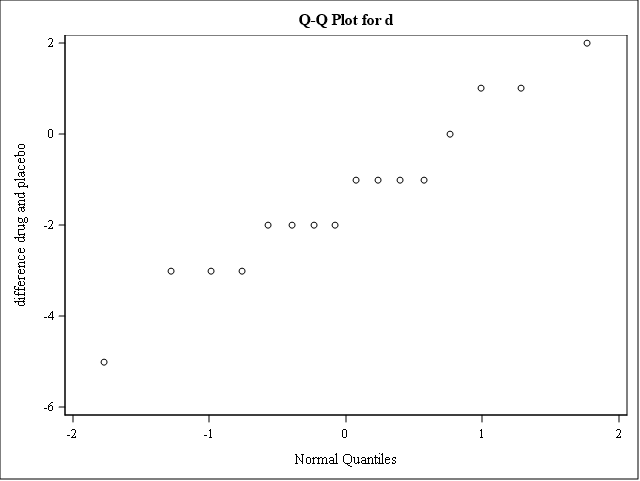
\includegraphics[width = 0.6\textwidth]{qqplot.png}
\end{center}

\item The two treatments (music and no music) should be assigned randomly in 2 periods of the experiment. In this way we can balance out some potential bias.



		\end{enumerate}

\newpage
		\item 
\begin{enumerate}
	\item 
	\begin{enumerate}
		\item  it is a randomized complete block experiment.
		\item experimental units: all plots of a certain kind of crop.

		treatments: six plant densities. (7, 8, 9, 10, 11, and 12 $\textrm{plant}/m^2$)

		blocks: five fields with different soil fertility.


		\item \

		\begin{center}
		\begin{tabular}{lll}
		\toprule
		Source & DF & Sums of Squares\\
		\midrule
		treatment & 5 & \\
		block & 4 & \\
		error & 20 &\\
		total & 29&\\
		\bottomrule

		\end{tabular}
		\end{center}
	\end{enumerate}

	\item 
	\begin{enumerate}
		\item
	it is a completely randomized experiment.
	\item experimental units: 15 different boards.

		treatments: three cutting speeds (50, 70, and 90 rpm).


		\item \

		\begin{center}
		\begin{tabular}{lll}
		\toprule
		Source & DF & Sums of Squares\\
		\midrule
		treatment & 2 & \\
		error & 12 &\\
		total & 14&\\
		\bottomrule

		\end{tabular}
		\end{center}
	\end{enumerate}

	\item 
	\begin{enumerate}
		\item  it is a randomized complete block experiment.
		\item experimental units: all workers in 8 plants.

		treatments:  four distinct music programs and no music.

		blocks: 8 plants.


		\item \

		\begin{center}
		\begin{tabular}{lll}
		\toprule
		Source & DF & Sums of Squares\\
		\midrule
		treatment & 4 & \\
		block & 7 & \\
		error & 28 &\\
		total & 39&\\
		\bottomrule

		\end{tabular}
		\end{center}
	\end{enumerate}
\end{enumerate}



\newpage
		\item 
		\begin{enumerate}
			\item \ 

			\begin{center}
			\begin{tabular}{llllll}
			\toprule
			Source&DF&Sum of Squares&Mean Square&$F$ Value&$Pr > F$\\
			\midrule
Subject&14&371.5066667&26.5361905&18.45&$<.0001$\\
Feet Placement&2&91.6000000&45.8000000&31.84&$<.0001$\\
Error&28&40.2733333&1.4383333&&\\
Corrected Total&44&503.3800000&&	\\
\bottomrule
\end{tabular}
\end{center}

\item 
Significant differences in mean torque for the three feet placements is determined
through testing for the treatment effect (feet placements). The $F$-test from the ANOVA Table
gives the $F$ statistic value as 31.84 with a p-value of $< 0.0001$. This means there 
is a statistically significant difference in the mean torque levels for the three feet placements.


\item 
Below is the output for the Tukey HSD method for pairwise comparisons
of the treatment means. In this case, the mean torque when feet placement is neutral is significantly different from the mean torque for other two feet placements with the highest mean torque level. There is no significant differencce in the mean torque for feet placements of back and staggered.

\begin{center}
\begin{tabular}{llll}
\toprule
Tukey Grouping& Mean&N&Feet Placement\\
\midrule
A&24.1000&15&N\\
B&21.7000&15&B\\
B&20.7000&15&S\\
\bottomrule
\end{tabular}
\end{center}

\item 
Two contracts used are $- \mu_B + \mu_S$ and $-\mu_B + 2 \mu_N - \mu_S$. We can see $-1 + 1 = 0$ and $-1 + 2 -1 = 0$, so they are contrast. Also, $(-1)\cdot (-1) + 0 \cdot 2 + 1 \cdot (-1) = 0$, thus they are orthogonal contrasts. 

\begin{center}
	\begin{tabular}{llllll}
	\toprule
Contrast&DF&Contrast SS&Mean Square&$F$ Value&$Pr > F$\\
\midrule
$-\mu_B + \mu_S$&1&7.50000000&7.50000000&5.21&0.0302\\
$-\mu_B + 2 \mu_N - \mu_S$&1&84.10000000&84.10000000&58.47&$<.0001$\\
\bottomrule
	\end{tabular}
\end{center}

The $F$-test statistic for the $-\mu_B + \mu_S$ contrast is 5.21 with a pvalue
$0.032$ and for the $-\mu_B + 2 \mu_N - \mu_S$ contrast is 58.47 with a p-value $<
0.0001$. This means that  $-\mu_B + 2 \mu_N - \mu_S$ is significantly different from 0, which supports the result in (c). The p-value for $-\mu_B + \mu_S$ is also low, but it is much bigger then that of $-\mu_B + 2 \mu_N - \mu_S$. We can still conclude that $-\mu_B + \mu_S$ is significantly different than 0, which does not support (c).


\item 
The normal probability plot suggests the residuals are from a normal
distribution, because the values arein a straight line.
\begin{center}
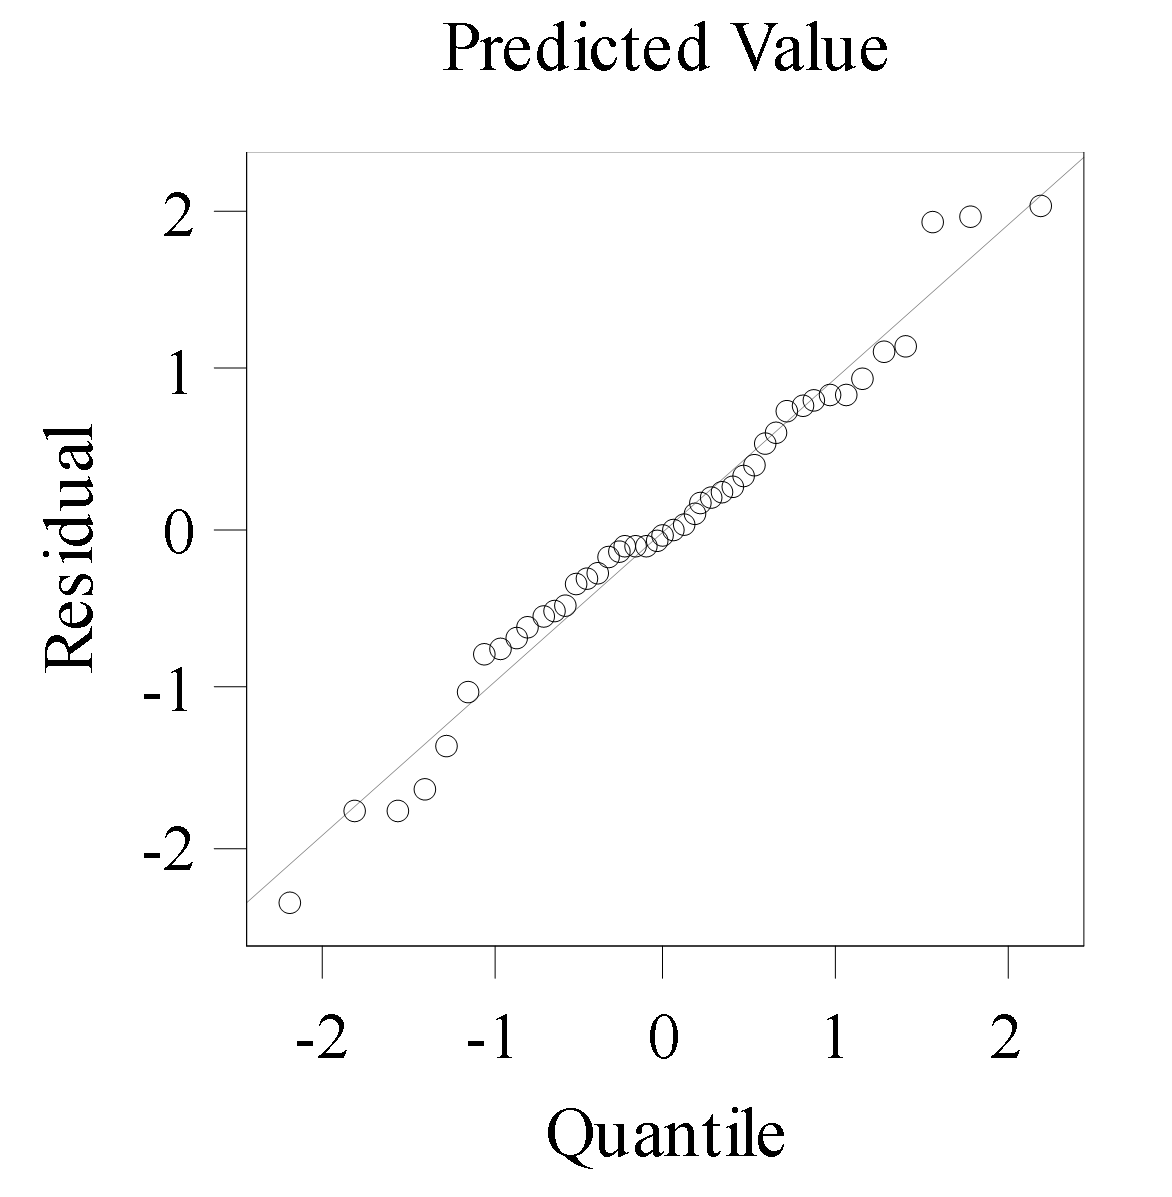
\includegraphics[width = 0.4\textwidth]{resqq.png}
\end{center}


\item 
The residuals in this plot should be randomly scattered, but there appears to be a
pattern. The residuals for low and high predicted values are positive, and the
residuals for many of the middle predicted values are negative or positive. This indicates that
the model is not capturing some particular feature of the data. 
\begin{center}
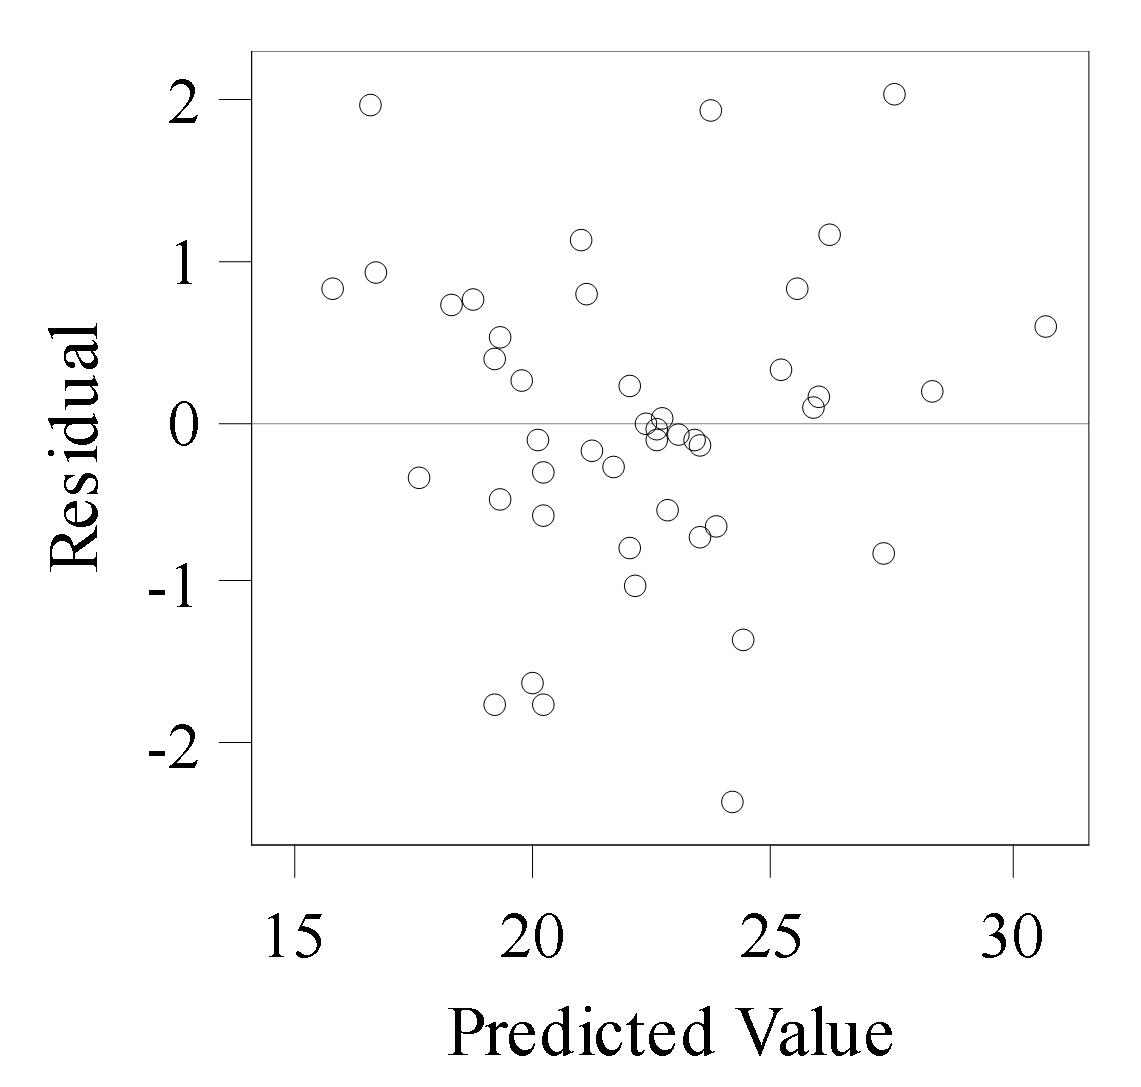
\includegraphics[width = 0.4\textwidth]{resvspredict.png}
\end{center}

\item 
 \[\hat{\sigma}_{CRD} = \frac{(n-1) MS_{blocks} + n (J-1) MS_{error}}{nJ - 1} = \frac{14 \times 26.54 + 15 \times 2 \times 1.44}{15\times 3 -1} = 9.43\]

 \[\hat{\sigma}_{RCBD} = MS_{error} = 1.44\]

 \[\textrm{Estimated Efficiency} = \frac{(28 + 3) 9.43}{(28 + 1) 1.44} = 7.00\]

 This means to have the same efficiency, $n_{CRD} = 7.00 n_{RCBD}$. Thus blocking is a efficient method in this case.
		\end{enumerate}
		
\end{enumerate}
	
	\end{document}